\documentclass{article} 


%% PACKAGES QUE USE, APARTE DE LOS OBVIOS COMO FLOAT, GRAPHICX, AMSMATH, BABEL
\usepackage{graphicx}
\usepackage{amsmath}
\usepackage{units} % permite usar nicefrac 
\usepackage{url}   % para poner links


\begin{document}
\section{Sample and hold}
La etapa de sample and hold, o track and hold, cumple la funci\'on de mantener la se\~nal constante por un tiempo suficiente como para medir su valor. Este proceso se divide en dos:
\begin{itemize}     
	\item \underline{Sample o track:} la salida es igual a la entrada.     
	\item \underline{Hold:} la salida se mantiene constante en el valor que ten\'ia cuando se recibi\'o la se\~nal de hold. 
\end{itemize}

Para este fin se utiliz\'o, de acuerdo a lo pautado por la c\'atedra, el integrado LF398\footnote{Hoja de datos consultada: \url{http://www.ti.com/lit/ds/symlink/lf398-n.pdf}.}. Al mismo se lo controla con una se\~nal cuadrada: cuando la misma toma un valor superior al de la referencia l\'ogica (con un threshold de 1.4V) se opera en modo sample, y con valor inferior a la referencia, en modo hold. Sus principales limitaciones est\'an dadas por:    
\begin{itemize}      
	\item La salida debe mantenerse dentro de los valores de tensi\'on de la alimentaci\'on.      
	\item Para frecuencias bajas debe tenerse en cuenta el droop rate, es decir qu\'e tan r\'apido se descarga el capacitor de hold.      
	\item Para frecuencias altas, pueden surgir problemas con el slew rate y/o con el tiempo de establecimiento  y de adquisici\'on de la se\~nal en hold.   
\end{itemize}   

Para satisfacer los requerimientos que se tengan en frecuencia, se debe elegir el capacitor de hold apropiadamente. Esto se debe a que cuanto mayor sea el capacitor, m\'as estable ser\'a la se\~nal de salida (se reducir\'an el droop rate y el tiempo de establecimiento), pero el sistema ser\'a m\'as lento a cambios en la entrada en el momento de sample (empeorar\'a el tiempo de adquisici\'on). Un droop rate elevado impide trabajar a bajas frecuencias, mientras que cuanto mayores sean los tiempos de adquisici\'on y establecimiento, menor ser\'a la m\'axima frecuencia a la que el integrado funciona correctamente. \par

Se procedi\'o, pues, a realizar mediciones de tiempo de establecimiento y tiempo de adquisici\'on con distintos capacitores (tabla \ref{table:sh_mediciones}). En cuanto al droop rate, dado que al computar la derivada de la tensi\'on, se arrojaban valores poco representativos de la se\~nal debido a la presencia de ruido, se decidi\'o utilizar los valores de la hoja de datos del integrado para realizar la comparaci\'on. Se utiliz\'o el gr\'afico proporcionado por el fabricante, que se observa en la figura \ref{fig:droop_rate}.


\begin{table}[htb]     
	\centering     
	\begin{tabular}{|c|c|c|}         
	\hline         Capacidad & Tiempo de establecimiento (s) & Tiempo de adquisici\'on (s)  \\ \hline \hline         
	100pF     & $9\times 10^{-7}$             & $1.4\times 10^{-6}$                                   \\ \hline         
	10nF      & $\leq 1.3\times 10^{-8}$      & $8.0\times 10^{-6}$                                                   \\ \hline
	100nF     & $\leq 1.3\times 10^{-8}$      & $1.3\times 10^{-4}$                                                 \\ \hline
    \end{tabular}     
	\caption{Par\'ametros del LF398 para distintos valores de $\mathrm{C}_\mathrm{h}$}     
	\label{table:sh_mediciones} 
\end{table}

\begin{figure}[htb]     
	\centering     
	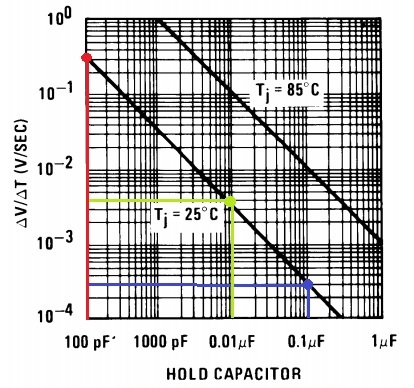
\includegraphics[scale=0.7]{sh/droop_rate.jpg}     
	\caption{Droop rate en funci\'on de $C_h$ para el LF398}     
	\label{fig:droop_rate} 
\end{figure}

En primer lugar, cabe aclarar que las mediciones de tiempo de establecimiento se vieron limitadas por los instrumentos de medici\'on utilizados: puesto que el rise time del generador utilizado para realizar las mediciones es de 13ns, es imposible con este instrumento medir un tiempo de establecimiento del mismo orden que este valor. Sin embargo, s\'i se pudo realizar esta medici\'on para el capacitor m\'as peque\~no.\par

Resulta claro de estas mediciones que el capacitor de 100nF, por su tiempo de adquisici\'on, no permitir\'ia trabajar con frecuencias mayores a aproximadamente 3.5kHz con duty del 50\%, lo cual es inaceptable considerando que $f_p=1.5$kHz: s\'olo se podr\'ia muestrear en el l\'imite establecido por el teorema de Nyquist, casi sin margen de error alguno. Con este capacitor, adem\'as, se hace demasiado notorio el problema de la absorci\'on diel\'ectrica, por el cual en la etapa de hold el capacitor tiende a volver al valor de hold anterior. Este efecto se observa en la figura \ref{fig:1k6}. \par

\begin{figure}[htb]     
	\centering     
	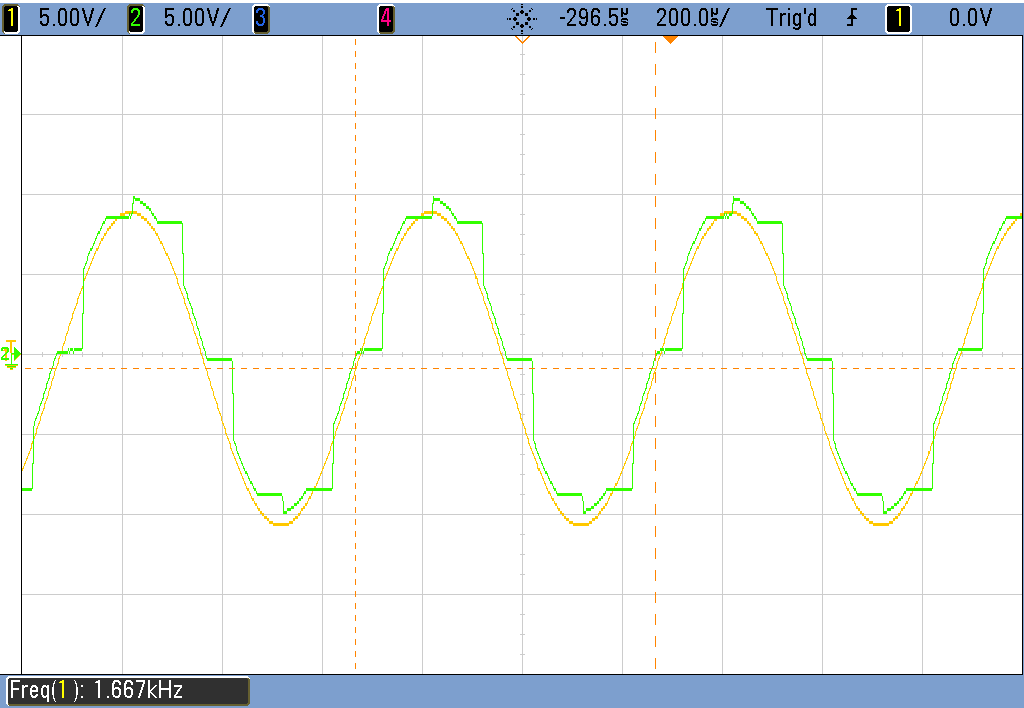
\includegraphics[scale=0.25]{sh/1k6_100p.png}     
	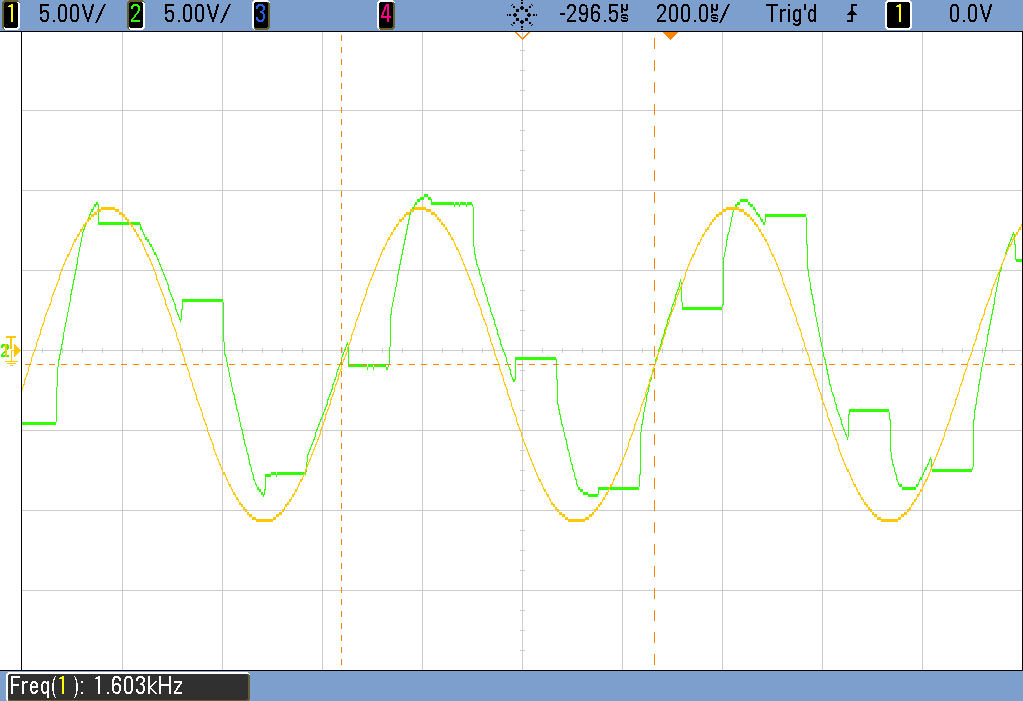
\includegraphics[scale=0.25]{sh/1k6_100n.png}     
	\caption{Salida del sample and hold (verde) con entrada senoidal de 1.6KHz (amarillo). Izquierda: capacitor de 100pF. Derecha: capacitor de 100nF.}     
	\label{fig:1k6} 
\end{figure}

Por otro lado, con el capacitor de 100pF, si bien los tiempos medidos fueron peque\~nos, esto es en desmedro de la estabilidad de la se\~nal en hold. En la figura \ref{fig:240k}, se observa c\'omo para frecuencias elevadas el capacitor no mantiene correctamente el valor de la se\~nal. En cuanto al droop rate documentado para este valor de $\mathrm{C}_\mathrm{h}=$100pF, de $0.3\nicefrac{V}{s}$, provocar\'ia que caiga 1.2mV trabajando a 500Hz con 50\% de duty, que es la m\'inima frecuencia sub nyquist que se utilizar\'a, con lo cual en principio esto no deber\'ia ser un problema. 

\begin{figure}[htb]     
	\centering     
	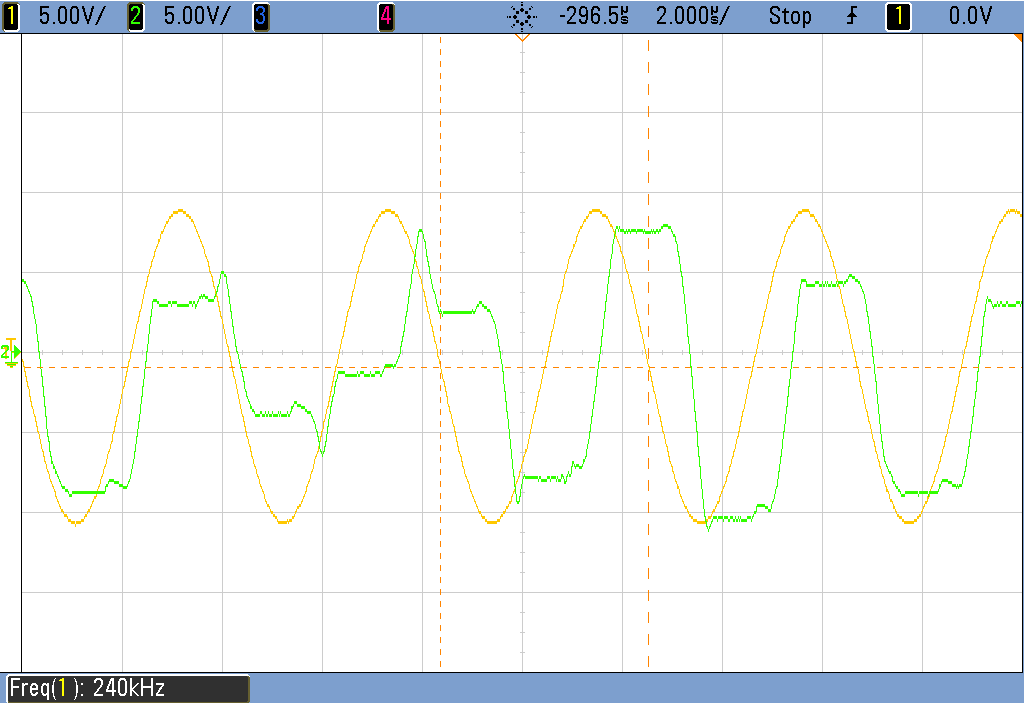
\includegraphics[scale=0.25]{sh/240k_100p.png}     
	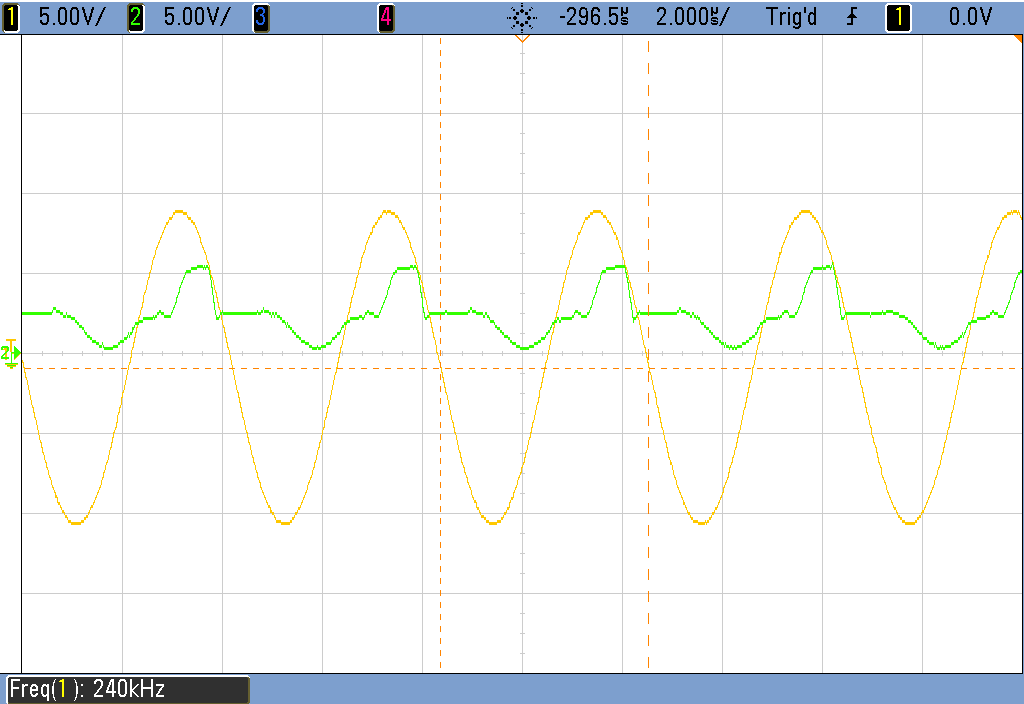
\includegraphics[scale=0.25]{sh/240k_100n.png}     
	\caption{Salida del sample and hold (verde) con entrada senoidal de 240KHz (amarillo). Izquierda: capacitor de 100pF. Derecha: capacitor de 100nF.}     
	\label{fig:240k} 
\end{figure}

Por \'ultimo, con el capacitor de 10nF recomendado por el fabricante, se consigue un droop rate de 4mV/s, completamente despreciable para nuestra aplicaci\'on, mientras que la frecuencia m\'axima a la que se puede trabajar sube a 62.5kHz, lo cual permite tomar 40 muestras por per\'iodo de una se\~nal con $f_{in}=f_p$. Con este capacitor, adem\'as, la se\~nal resulta mucho menos ruidosa que la del capacitor de 100pF. Por lo tanto, este es el valor que se decidi\'o utilizar.

\begin{figure}[htb]     
	\centering     
	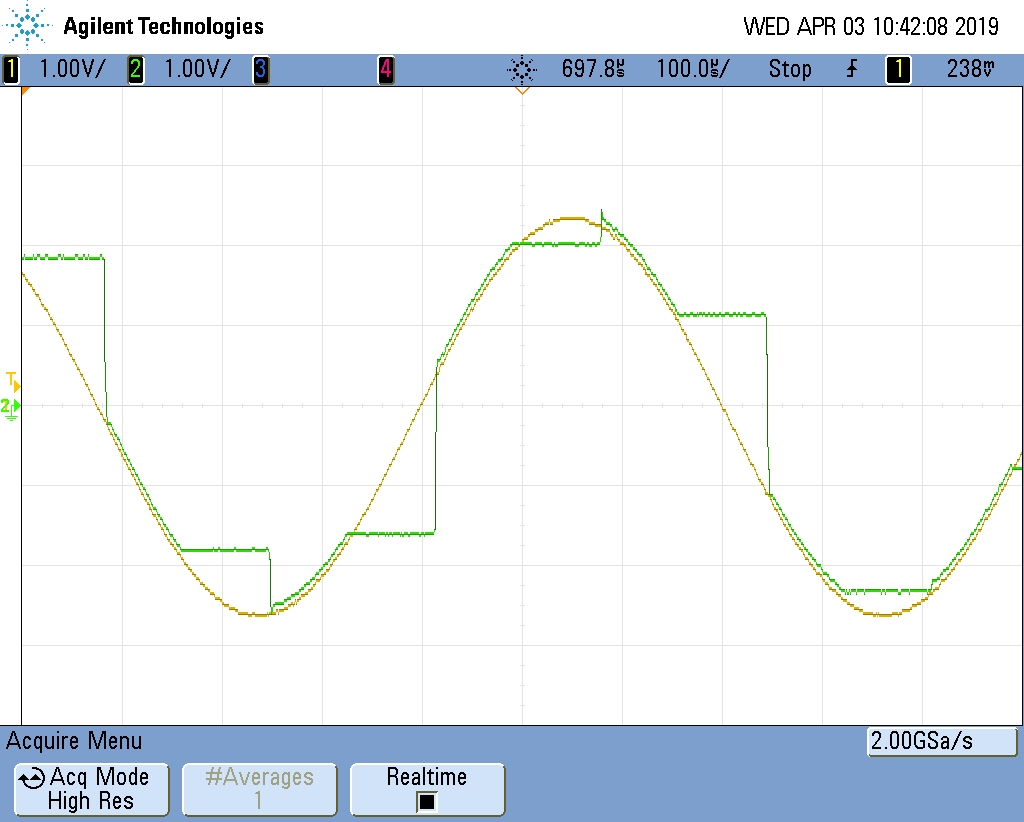
\includegraphics[width=0.5\textwidth]{sh/sh_10n.png}     
	\caption{Salida del sample and hold (verde) con entrada senoidal de 1.6KHz (amarillo). Capacitor de 10nF.}     	
	\label{fig:sh_10n} 
\end{figure}

En cuanto a la tecnolog\'ia de este componenete, se sigui\'o tambi\'en la recomendaci\'on del fabricante de usar un capacitor film, debido a que su diel\'ectrico tiene bajas p\'erdidas y mejor comportamiento en cuanto a absorci\'on diel\'ectrica que en otros tipos de capacitores.

En la figura \ref{fig:sh_10n}, se observa c\'omo se comporta el integrado con el capacitor elegido. La se\~nal se ve mucho m\'as estable en hold que para el capacitor de 100pF, sin los problemas de absorci\'on diel\'ectrica manifestados por el de 100nF.

\end{document}